\documentclass[pdflatex,sn-mathphys-num]{sn-jnl}
\usepackage{graphicx}%
\usepackage{multirow}%
\usepackage{amsmath,amssymb,amsfonts}%
\usepackage{amsthm}%
\usepackage{mathrsfs}%
\usepackage[title]{appendix}%
\usepackage{xcolor}%
\usepackage{textcomp}%
\usepackage{manyfoot}%
\usepackage{booktabs}%
\usepackage{algorithm}%
\usepackage{algorithmicx}%
\usepackage{algpseudocode}%
\usepackage{listings}%
\usepackage{float}


\theoremstyle{thmstyleone}
\newtheorem{theorem}{Theorem}
\newtheorem{proposition}[theorem]{Proposition}% 

\theoremstyle{thmstyletwo}%
\newtheorem{example}{Example}%
\newtheorem{remark}{Remark}%

\theoremstyle{thmstylethree}%
\newtheorem{definition}{Definition}%

\raggedbottom


\begin{document}

\title[Article Title]{LLMBot: Multi-Agent Robotic Systems for Adaptive Task Execution}



\author{\fnm{Harith} \sur{Ibrahim}}\email{harithsami01@gmail.com}


\author{\fnm{Harith} \sur{Alsafi}}\email{harith.alsafi@gmail.com}
\author{\fnm{Shane} \sur{Xi}}\email{S.Q.Xie@leeds.ac.uk}


\affil{\orgdiv{School of Electrical and Electronics Engineering}, \orgname{University of Leeds}, \orgaddress{\city{Leeds}, \state{West Yorkshire}, \country{United Kingdom}}}



% make everything past tense

\abstract{Robotic task planning systems often require significant computational and financial cost, limiting their accessibility and scalability. Can we leverage recent advancements in Large Language Models (LLMs) to create more cost-effective and lightweight robotic planning solutions? This paper introduces a framework that integrates LLMs with robotic systems for natural language interaction and task execution. Our approach, which we call LLMBot (Large Language Model Robotic Planner), combines GPT-3.5 Turbo for natural language understanding, reasoning, and high-level task planning with a simulated 3D environment in Unreal Engine. LLMBot uses behavior trees for robust low-level execution of robotic actions, grounding the LLM’s capabilities in a practical robotic context. The system employs prompt engineering, multimodal input, and parameter optimization to enhance the LLM’s performance and reduce computational overhead. For systematic evaluations, we developed a comprehensive test suite assessing success rates, spatial distributions, and cost-effectiveness across various scenarios. Experimental results demonstrate that our approach outperforms traditional planning systems in terms of computational efficiency and cost-effectiveness while maintaining comparable task success rates. Additionally, we have demonstrated LLMBot capabilities within simulated environments. This research advances multi-agent collaboration and human-robot interaction by enabling more intuitive and resource-efficient communication between humans and robots. By combining modern language models with lightweight 
execution frameworks, this project paves the way for more accessible, adaptive, and cost-effective robotic solutions capable of natural language-based collaboration
}


\keywords{Robotic Task Planning, Large Language Models (LLMs), Natural Language Interaction, Cost-Effective Robotic Solutions}


\maketitle


\section{Introduction}\label{sec1}
Effective robotic task planning requires not only a deep understanding of the environment and available actions but also the ability to interpret and execute high-level, natural language instructions \cite{iovino2022survey}. Traditional approaches to robot planning often involve complex, expensive algorithms that are difficult to develop and maintain. It is possible to leverage recent advancements in large language models (LLMs) to create more accessible and cost-effective robot planning solutions\cite{vemprala2023chatgpt}. The work introduces LLMBot (Large Language Model Robotic Planner), a novel framework that integrates LLMs with symbolic planning methods for intuitive, natural language-based robot control.

LLMs with exensive comprehensive training data have demonstrated remarkable multi-task generalization and common-sense reasoning capabilities\cite{naveed2024comprehensive}. Recent research has explored their potential in robotic task planning by selecting a series of actions. However, these approaches often lack grounding in the robot's physical capabilities and current environmental state\cite{jiang2022vima}. LLMBot addresses this limitation by combining the rich language understanding of LLMs with the efficiency and adaptability of symbolic planners, specifically behavior trees.
\begin{figure}[H]
\centering
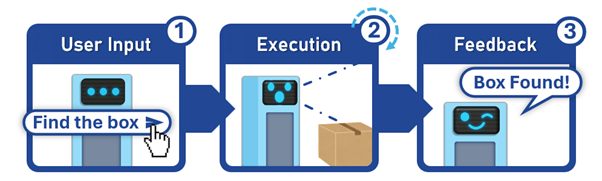
\includegraphics[width=0.7\textwidth]{figures/Picture13.png}
\caption{Diagram Showing Simplified Project Plan}\label{fig1}
\end{figure}

A key component of LLMBot is its use of GPT-3.5 Turbo for natural language understanding, reasoning, and high-level task planning. The context memory of LLMs was leveraged to include the history of recent actions, environment objects, and function definitions for tasks. It incorporates situational awareness to it by asserting preconditions and implementing recovery actions for failed assertions. LLMBot operates within a simulated 3D environment in Unreal Engine, allowing for comprehensive testing and evaluation. The system utilizes behavior trees for robust low-level execution of robotic actions, bridging the gap between high-level language understanding and concrete robot behaviors. We employ prompt engineering, multimodal input, and parameter optimization to enhance the LLM's performance and reduce computational overhead.
\vfill

Our approach goes beyond simple language-to-action mapping. LLMBot enables robots to interpret complex, free-form natural language instructions, reason about the given task, and coherently execute the necessary actions to accomplish the objective. Moreover, it exhibits adaptability to handle novel situations without extensive retraining or reprogramming. To evaluate LLMBot, we developed a comprehensive test suite assessing success rates, spatial distributions, and cost-effectiveness across various scenarios. We also showcase LLMBot's capabilities using autonomous robots in simulated environments in Unreal Engine, highlighting its potential for real-world applications.

This research advances multi-agent collaboration and human-robot interaction by enabling more intuitive and resource-efficient communication between humans and robots. By combining modern language models with lightweight execution frameworks, LLMBot paves the way for more accessible, adaptive, and cost-effective robotic solutions capable of natural language-based collaboration.

Our key contributions include:
\begin{itemize}
    \item The novel combination of GPT-3.5 Turbo for high-level cognition and behavior trees for low-level action execution, enabling natural language command interpretation in a simulated 3D environment.
    \item A comprehensive evaluation demonstrating LLMBot's  flexibility and natural language understanding compared to traditional robotic planning techniques.
    \item A hierarchical multi-agent setup showcasing the system's potential for coordinating complex tasks.
\end{itemize}
\section{Background and Related Work}

\subsection{Task Planning in Robotics}
Task planning in robotics has traditionally relied on symbolic AI techniques, involving the use of formal logic and search algorithms to generate sequences of actions that achieve specified goals. These approaches, while powerful, often struggle with scalability in complex, real-world environments due to the overwhelming increase in potential states and actions \cite{iovino2022survey}).

Recent advancements have seen the integration of learning-based methods with classical planning techniques. For instance, Karpas and Magazzeni (2020) survey the landscape of planning in artificial intelligence, highlighting the trend towards hybrid systems that combine the strengths of both symbolic and learning-based approaches \cite{annurev:/content/journals/10.1146/annurev-control-082619-100135}.

\subsection{Large Language Models in AI and Robotics}
Large Language Models (LLMs) have emerged as a transformative technology in artificial intelligence, demonstrating remarkable capabilities in natural language understanding and generation. These models, exemplified by GPT-3 \cite{brown2020languagemodelsfewshotlearners}, are trained on a large set of text data, enabling them to capture complex patterns of language use and exhibit behaviors that appear to mimic reasoning and common sense understanding \cite{naveed2024comprehensive}.

The potential application of LLMs to robotics and embodied AI has garnered significant attention in recent years. Researchers have begun exploring how the rich language understanding and generation capabilities of LLMs can be leveraged to enhance robotic task planning and execution. For instance,\cite{huang2022largelanguagemodelsselfimprove} demonstrate the use of LLMs for generating task plans in simulated robotic environments, showcasing the potential for these models to bridge the gap between natural language instructions and low-level robot actions.

\subsection{Embodied AI and Grounding}
A critical challenge in applying LLMs to robotics is the problem of grounding – connecting abstract language representations to concrete, physical actions and perceptions. This challenge has been a long-standing issue in AI and robotics, dating back to early work on symbol grounding \cite{HARNAD1990335}.

Recent work has explored various techniques to enhance LLMs' capabilities for embodied environments:

\begin{itemize}
    \item \textbf{Prompt Engineering:} Carefully crafting input prompts to guide LLM outputs towards desired behaviors, effectively defining the operational context and constraints \cite{liu2023llmpempoweringlargelanguage}.
    
    \item \textbf{Multimodal Integration:} Incorporating visual, auditory, or other sensory data alongside text inputs to provide richer contextual information to the model \cite{jiang2022vima}.
    
    \item \textbf{Few-Shot Learning:} Utilizing a small number of examples to rapidly adapt LLMs to new domains or tasks, a technique that has shown promise in improving model performance on specialized tasks \cite{brown2020languagemodelsfewshotlearners}.
\end{itemize}

\subsection{Symbolic Planning in Robotics}
While learning-based methods have gained prominence, symbolic planning techniques remain crucial in robotics due to their interpretability and formal guarantees. Behavior Trees, for instance, offer a flexible and modular approach to defining robot behaviors \cite{JIANG2022100869}. The integration of symbolic planning with learning-based approaches represents a promising direction for robotic task planning \cite{koyama2022study}. 

\subsection{Challenges and Open Problems}
Despite recent progress, several challenges remain in the application of LLMs to robotic task planning:

\begin{itemize}
    \item \textbf{Hallucination and Consistency:} LLMs can generate plausible but incorrect information, a phenomenon known as hallucination. Ensuring consistency and reliability in robot-critical applications remains an open problem \cite{yang2023plug}.
    
    \item \textbf{Ethical Considerations:} The use of LLMs in robotics raises important ethical questions, particularly regarding bias, privacy, and the potential for misuse. Addressing these concerns is crucial for the responsible development of LLM-based robotic systems \cite{chen2023frugalgptuselargelanguage}.
\end{itemize}

As the field continues to evolve, addressing these challenges while leveraging the unique capabilities of LLMs presents opportunities for advancing robotic task planning and execution.



\section{Method}
The LLM integration is demonstrated with behavior trees, robot abilities definitions, and deploys the approach in a virtual Unreal Engine environment for household and industrial scenarios.

\subsection{Integration of Language Models and Behavior Trees}
The natural language understanding and high-level task planning is combined  with behavior trees to create a flexible and powerful decision-making framework for robotic agents. Specifically, the LLM:


\begin{itemize}
    \item Interprets natural language instructions and interprets goals.
    \item Examines environment condition, robot current state and world context.
    \item Creates a low-level plan from the provided behaviour set.
    \end{itemize}
    

\begin{figure}[H]
\centering
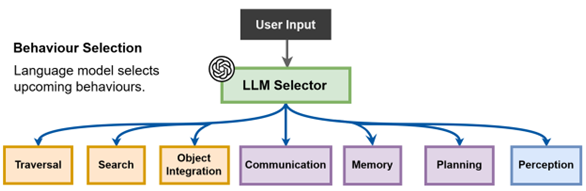
\includegraphics[width=0.6\textwidth]{figures/Picture12.png}
\caption{Proposed approach of utilizing Language Models in Behaviour Trees.}\label{fig7}
\end{figure}
Following recent work, we use prompting techniques such as zero-shot and few-shot learning, chain of thought reasoning, and multimodal prompting to enhance the model's performance. The behavior trees provide a hierarchical and modular structure for representing complex behaviors, making them easy to design, debug, and maintain.
\newpage
\subsection{Virtual World Implementation}
Given the integrated LLM and behavior tree framework. A Python environment was utilzied  to handle the LLM's logic and reasoning capabilities, which communicates sensor data and user inputs with the Unreal Engine simulation via a REST API. (shown in figure \ref{software}).
\begin{figure}[H]
\centering
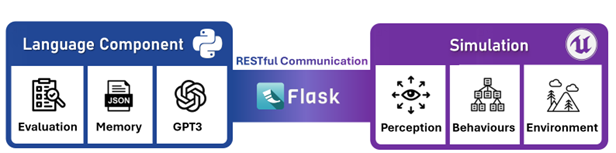
\includegraphics[width=0.9\textwidth]{figures/Picture2.png}
\caption{High level diagram of system architecture.}\label{software}
\end{figure}

The Unreal Engine environment provides a realistic testbed for our approach, leveraging its strengths in intelligent agent creation, behavior simulation, navigation, and perception systems.

Our approach enhances human-robot interactions by enabling robots to display appropriate emotional expressions based on the chat context. The system's modularity is emphasized through a JSON files, which are used to store conversation history, actions taken. It also allows for different robot abilities and configurations allowing for easy component replacement without modifying the underlying code.
This implementation allows us to test and evaluate our approach across diverse scenarios, assessing the system's performance in both household and industrial settings. 


The robots operate within a simulated warehouse environment, which consists of multiple rooms and different paths connecting them. This environment is designed to test the robots' ability to navigate and search effectively. The environment is also filled with various objects that the robots can interact with, in terms of manipulation or direct usage. This environment serves as a sandbox or testing ground, where users can request task-specific commands that the robots need to interpret correctly, given the current world context. 

Additionally, the environment provides a showcase of potential real-life implementation for warehouse automation.
Users can interact with the robots by navigating a humanoid avatar that navigates and interacts with the world. When in close proximity to the robots, a user interface appears, allowing for clear and user-friendly communication. The user interface consists of the following components:
\begin{figure}[H]
\centering
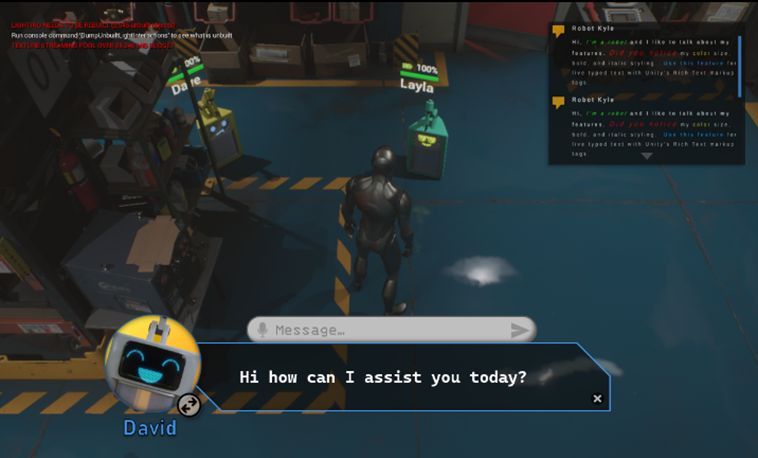
\includegraphics[width=0.7\textwidth]{figures/Picture9.png}
\caption{Screenshot showing Robot Chat User Interface.}\label{fig4}
\end{figure}
\begin{itemize}
\item \textbf{Chat Interface:} Located at the bottom of the screen, it takes in user messages in white text input, which also allows for microphone input for verbal user commands. The interface displays the robot's responses in a dark widget.
\item \textbf{Robot Avatar:} A circular icon representing the robot, positioned next to the responses. This avatar dynamically changes to reflect the robot's emotional state.
\item \textbf{Chat History:} A widget on the top left, showing prior conversations with the robot the user is currently talking to.
\item \textbf{Battery Display:} The robot's battery power percentage.
\end{itemize}

The interface and the environment are designed to be simple yet versatile, allowing for a wide range of scenarios to test the robot's planning generalization and ensuring ease of use for the user.


\subsection{Cost-Effective Planning and Simulated Environments}
A key challenge in robotic task planning is the development of sophisticated algorithms that are both effective and cost-efficient. Traditional approaches often require significant computational resources and financial cost, limiting their accessibility and scalability. Our work addresses this challenge by proposing a lightweight, LLM-integrated approach that reduces computational overhead while maintaining high task success rates.

Simulated environments are crucial in robotics research, allowing rapid prototyping and testing without physical hardware. LLMBot operates within a simulated 3D environment in Unreal Engine, enabling comprehensive evaluation across diverse scenarios. This setup assesses the system's performance, running costs, and cost-effectiveness in a controlled yet realistic setting.

The simulated environment models various sensors present on physical robots, including cameras, depth sensors, LiDAR, and proprioceptive sensors. This generates realistic sensory data mimicking real-world conditions. By integrating this multi-modal sensory information, we enable the LLM to reason about spatial relationships, identify objects and obstacles, and understand the robot's capabilities and limitations.

While our approach shows promise, challenges remain in areas like perception, navigation, and addressing potential hallucinations, biases, and ethical concerns in LLM outputs. Rigorous testing and evaluation are crucial to ensure reliability, safety, and trustworthiness in real-world applications.

Future work could explore the integration of more advanced LLM techniques, such as fine-tuning on domain-specific datasets or incorporating reinforcement learning to improve task execution over time. Additionally, investigating the scalability of this approach to more complex, multi-agent scenarios could open up new possibilities in collaborative robotics.

\subsection{Robot Abilities and Communication}
Our system implements robotic agents, called HelperBots, capable of navigating a virtual environment, interacting with objects, and performing various tasks based on natural language instructions. The HelperBots use six high-level behaviors as shown in Table \ref{robot-functions}:

\begin{table}[h]
\caption{Robot Functions and Use Cases}\label{robot-functions}
\begin{tabular*}{\textwidth}{p{72pt}p{113pt}p{60pt}}
\toprule
Function & Example use case & Function format \\
\midrule
go\_to & Go to the red room & \verb|go_to("red room")| \\
item\_interact & Pick up the bottle. & \verb|item_interact(Type.pick, "bottle")| \\
item\_search & Find the blue ball. & \verb|item_search("blue ball")| \\
item\_memory & Where is the cup? & \verb|item_memory("cup", Type.location)| \\
environment\_memory & What's the room temperature? & \verb|environment_memory("temperature")| \\
communicate & Tell Tom to "have a good day" & \verb|Communicate("Tom", "have a good day")| \\
\botrule
\end{tabular*}
\end{table}
\\For perception, we assume perfect object identification within the robot's line of vision. Navigation utilizes Unreal Engine's AI navigation system, employing a Navigation Mesh (NavMesh) for efficient pathfinding in the 3D environment.
The system employs two sets of memory , the first focusing on conversation/action history and the other stores and updates object-locations changes observed by the robot.

In terms of cross-robot communication, a "Master Robot" serves as a central control unit, with access to the combined memory of all other robots. This hierarchical architecture allows for efficient coordination and task allocation among specialized robots.

\begin{figure}[H]
\centering
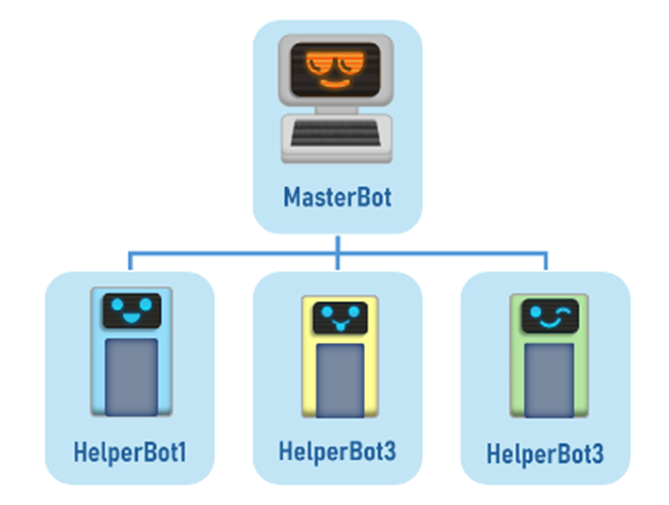
\includegraphics[width=0.5\textwidth]{figures/Picture6.png}
\caption{Diagram of robot command and memory hierarchy.}\label{hierarchy}
\end{figure}


\subsection{Cognitive Workflow}

Figure \ref{cognitive_loop} outlines the cognitive architecture for our LLM-driven robotic NPC, LLMBot. This system integrates a Large Language Model (LLM) with a Behavior Tree system and a Facial Expression Module to create a coherent NPC capable of cognition, communication, and action.
\begin{figure}[H]
\centering
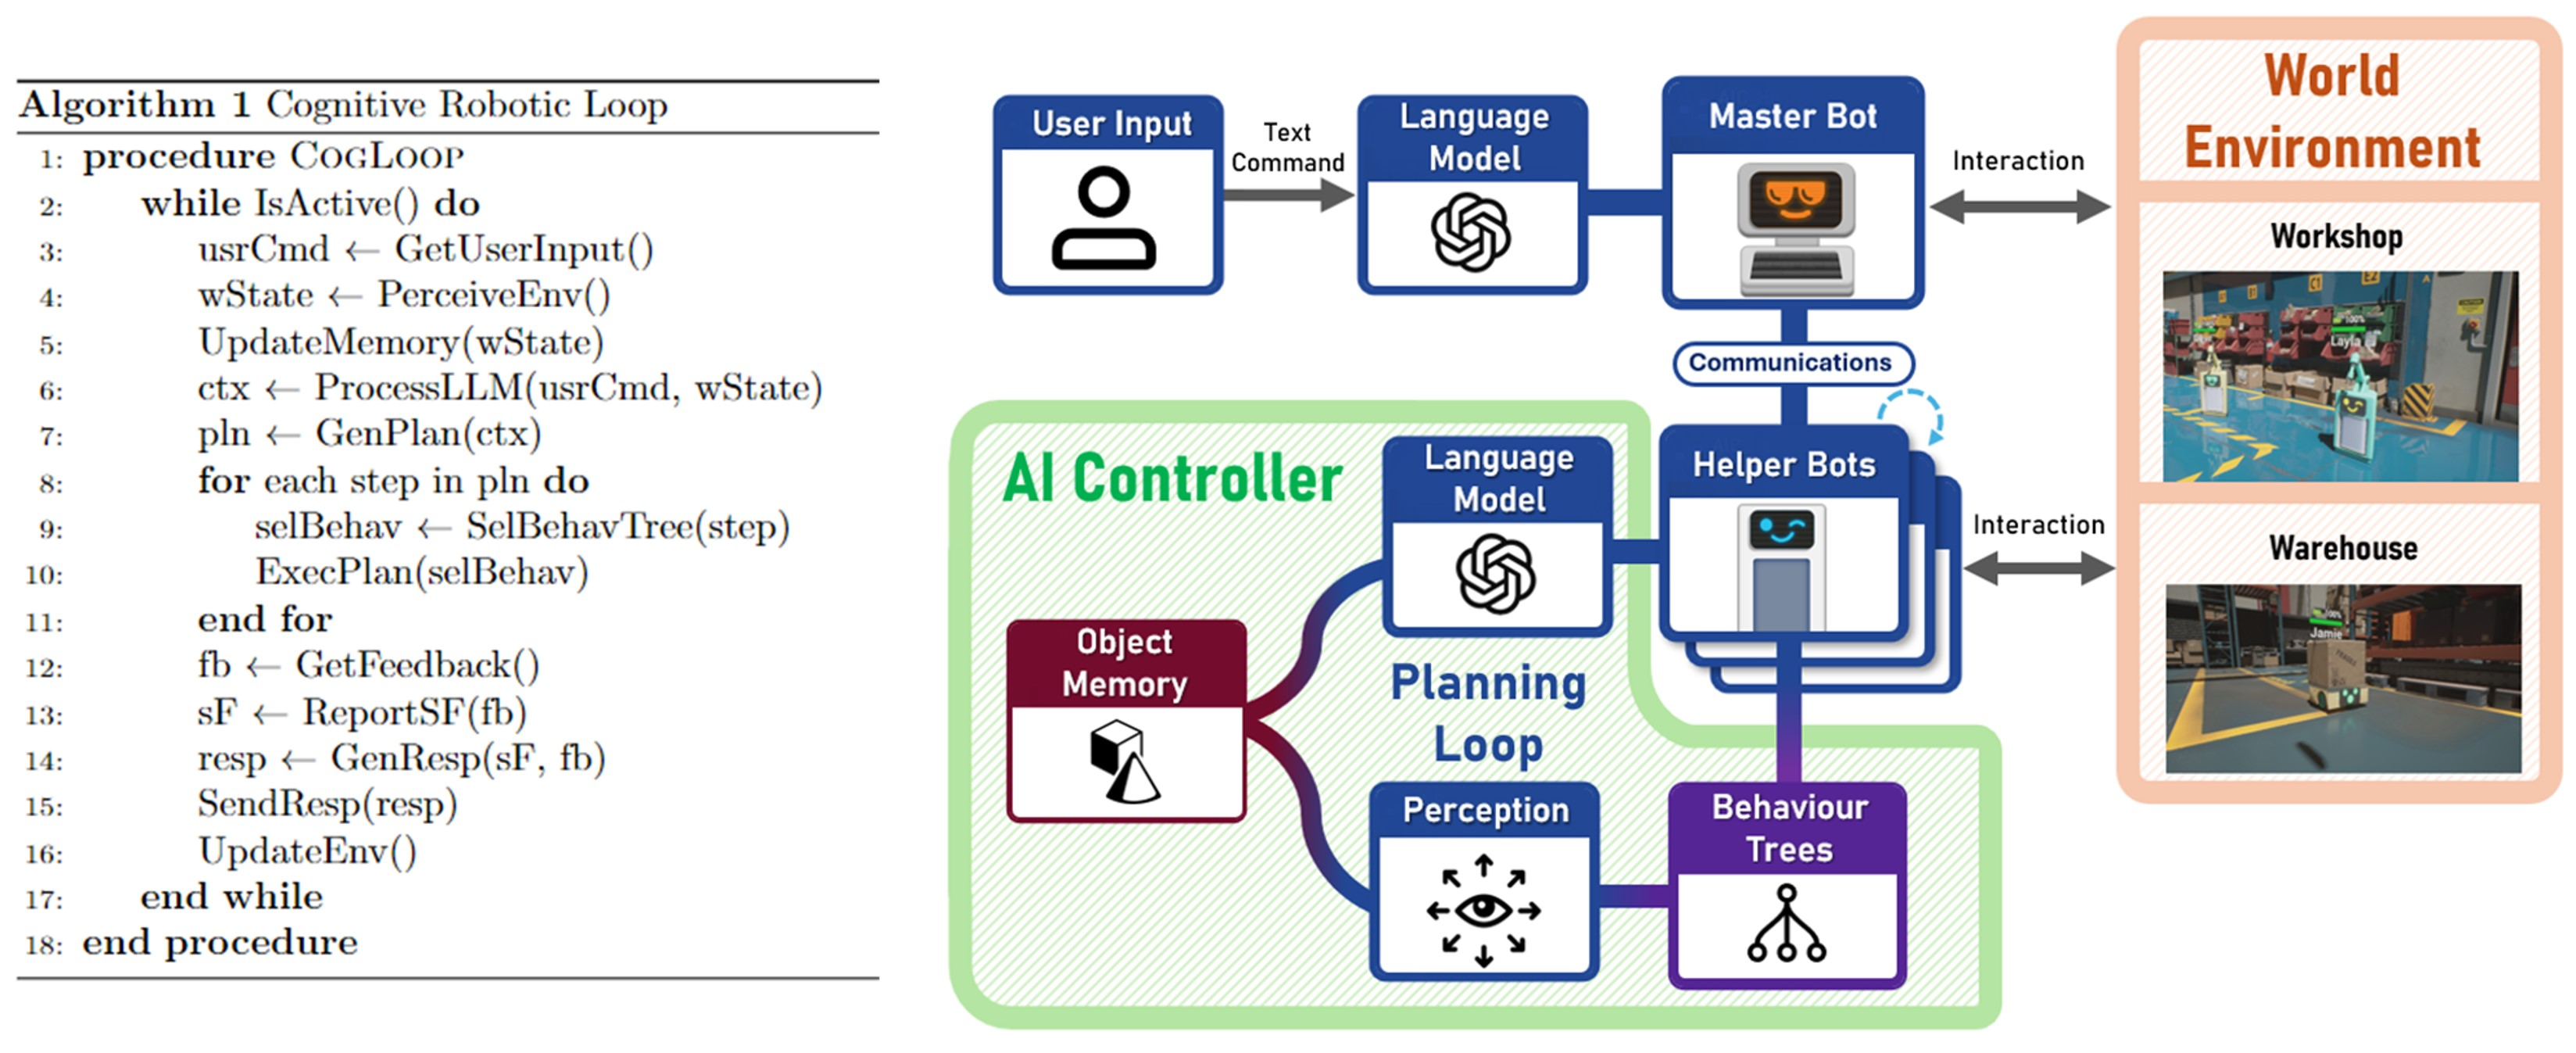
\includegraphics[width=1\textwidth]{figures/cognition.jpg}
\caption{Proposed Robot Cognitive Architecture.}\label{cognitive_loop}
\end{figure}

At the core of LLMBot's functionality is the Cognitive Robotic Loop, an advanced algorithm orchestrating the NPC's perception, reasoning, and action cycles. This continuous loop begins by updating the robot's internal world model with environmental data and user input. The LLM then processes this information to generate contextually appropriate responses and formulate a high-level action plan.
The system bridges abstract language understanding with concrete actions through a behavior tree, selecting and executing specific behaviors for each step of the plan. This hybrid approach ensures both flexibility in comprehension and reliability in execution.
Following action execution, the system evaluates its performance, generates feedback, and communicates with the user. The world model is then updated, completing the cognitive cycle. This iterative process enables LLMBot to maintain dynamic, contextually aware interactions, demonstrating cognitive flexibility akin to human-like interaction patterns.

The integration of LLM-based reasoning with robotic behaviors and emotional expressions represents a significant advancement in NPC design. This architecture successfully leverages the language understanding and generation capabilities of LLMs while grounding them in tangible actions and expressions. The result is a highly adaptable and responsive NPC system, capable of handling the complexities and open-ended nature of simulated environment interactions with unprecedented sophistication.
\newpage
\section{Experiments and Evaluation}
\subsection{Use Case Scenarios}


To evaluate the efficacy and versatility of our LLMBot framework, we implemented two complex use case scenarios demonstrating the system's capability to interpret and execute sophisticated natural language commands, both for single-robot and multi-robot collaborative tasks.
\begin{figure}[H]
    \centering
    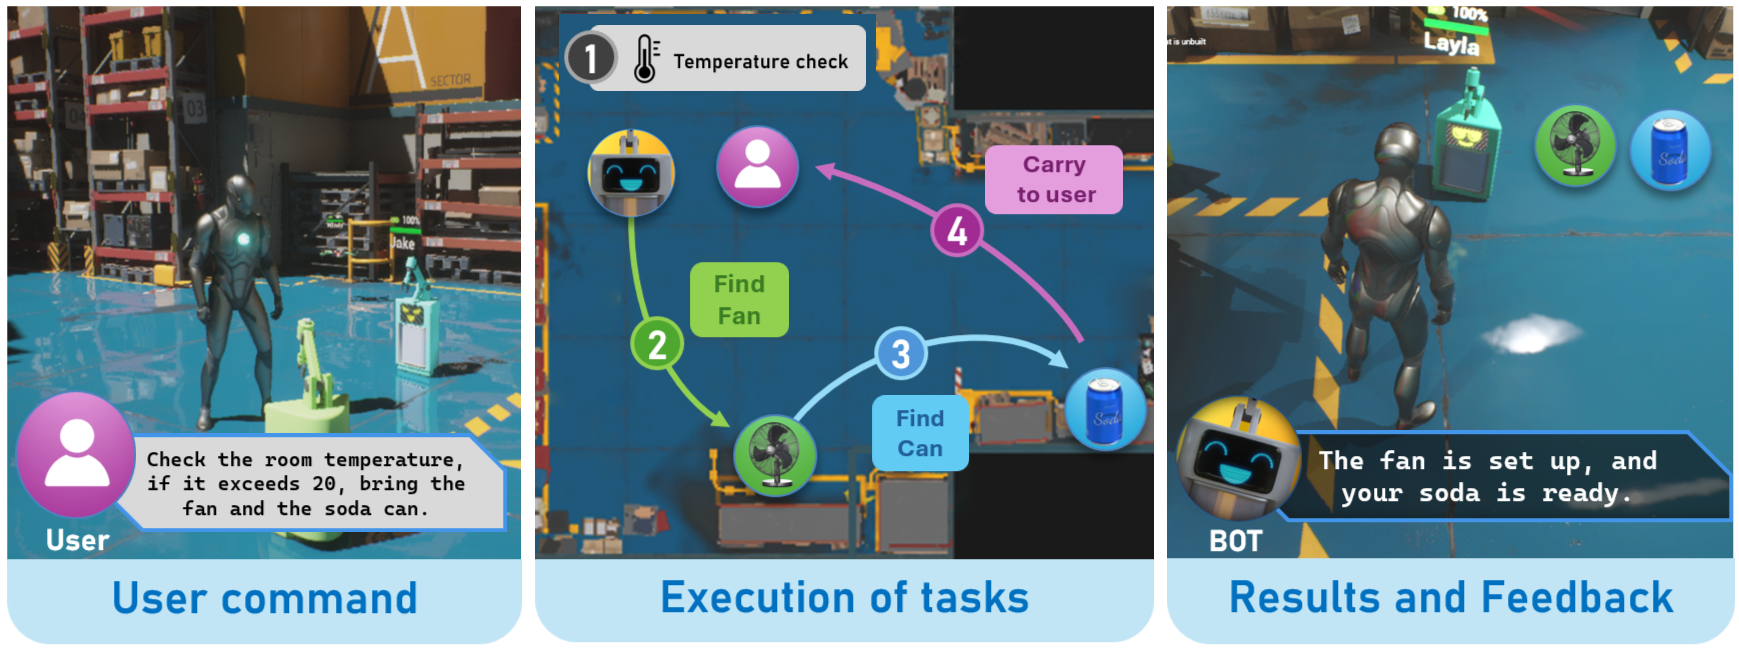
\includegraphics[width=1\textwidth]{figures/scenario1.png}
    \caption{Multi-step conditional task execution by a single robot}\label{scenario1}
    \end{figure}
    
Figure \ref{scenario1} illustrates the execution flow of a user command: "Check the room temperature, if it exceeds 20, bring the fan and the soda can." This command tests the system's ability to handle conditional logic, multi-step planning, and object interaction within the simulated environment. The LLMBot's cognitive process unfolds in three phases:
\begin{itemize}
    \item Command interpretation
    \item Task decomposition and planning
    \item Execution with feedback
\end{itemize}

The Large Language Model (LLM) component, utilizing GPT-3.5 Turbo, parses the natural language input, identifying key elements such as the conditional check, objects of interest, and implied actions. It then decomposes the command into actionable tasks, including temperature check, conditional evaluation, object localization, retrieval, and delivery. The system executes the plan using our behavior tree implementation in Unreal Engine, providing visual feedback throughout the process.
This scenario demonstrates several key strengths: natural language understanding, conditional logic processing, multi-step planning, object recognition and interaction, and user feedback. The system accurately interprets complex instructions, makes runtime decisions based on environmental data, and executes a coherent sequence of actions while providing clear, contextual feedback.

\begin{figure}[H]
    \centering
    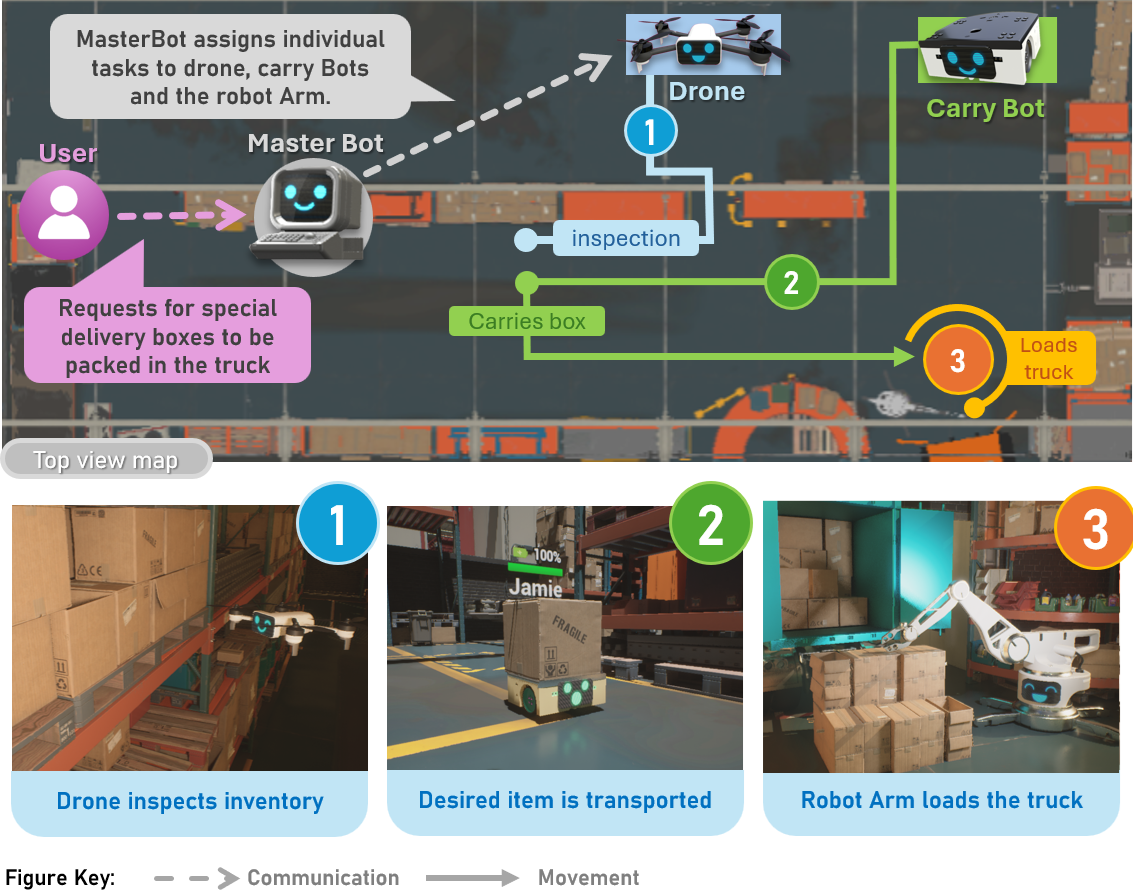
\includegraphics[width=1\textwidth]{figures/scenario2.png}
    \caption{Collaborative multi-robot task execution orchestrated by a Master Bot}\label{scenario2}
    \end{figure}
Figure \ref{scenario2} showcases a complex collaborative scenario involving multiple robotic agents, demonstrating the system's ability to orchestrate a coordinated response across multi-robotic platforms. The scenario begins with the user request:\\ \textbf{\textit{"Special delivery boxes to be packed in the truck."}} \\The Master Bot, powered by the LLM executes the following accordingly:
\begin{enumerate}
    \item \textbf{Command Interpretation and Task Distribution:} The Master Bot, powered by our LLM, interprets the user's request and formulates a comprehensive plan. It then decomposes this plan into subtasks, assigning them to the most suitable robotic agents:
    \begin{itemize}
        \item Drone: Tasked with inventory inspection
        \item Carry Bot: Assigned to transport the identified boxes
        \item Robot Arm: Designated for loading the truck
    \end{itemize}

    \item \textbf{Coordinated Execution:} The execution proceeds in a synchronized manner:
    \begin{itemize}
        \item The drone conducts an aerial inspection of the inventory, using computer vision to identify the "special delivery boxes."
        \item Based on the drone's findings, the Carry Bot retrieves and transports the identified boxes to the loading area.
        \item Finally, the Robot Arm, equipped for precise manipulation, loads the boxes into the truck.
    \end{itemize}

    \item \textbf{Continuous Communication and Adaptation:} Throughout the process, the Master Bot maintains communication with all agents, potentially adjusting the plan based on real-time feedback and changing conditions.
\end{enumerate}



The execution proceeds in a synchronized manner, with the drone conducting aerial inspection, the Carry Bot retrieving and transporting identified boxes, and the Robot Arm loading them into the truck. Throughout the process, the Master Bot maintains communication with all agents, potentially adjusting the plan based on real-time feedback and changing conditions.

This hivemind approach demonstrates several advanced capabilities: complex task decomposition, multi-agent coordination, optimal utilization of specialized robot capabilities, scalability to handle multi-step processes, adaptive planning with centralized control, and a natural language interface for initiating complex multi-agent operations.

Both scenarios exemplify the power of our LLMBot framework in bridging high-level cognitive tasks with practical robotic execution, whether for single-robot operations or multi-agent collaborations. By leveraging LLMs for complex reasoning and task distribution, combined with specialized execution frameworks, we achieve a highly flexible and efficient system capable of handling diverse tasks in real-world environments. This approach represents a significant advancement in robot cognition, multi-robot coordination, and human-robot interaction, paving the way for more intuitive and adaptable robotic solutions in various domains.

\newpage
\subsection{Evaluation Tests}


The evaluation approach aimed to comprehensively assess the system's performance, effectiveness, and the successful integration of classical robotics techniques with modern natural language processing methods in enabling smooth human-robot collaboration on complex tasks \cite{kruijff2007incremental}.
A sophisticated testing environment was developed, simulating a pastry factory operated by a swarm of robots under the coordination of a central MasterBot. The environment featured color-coded rooms, a kitchen area, an inventory management section, and a robot charging station, as shown in Figure \ref{simulation_environment}.
\begin{figure}[H]
\centering
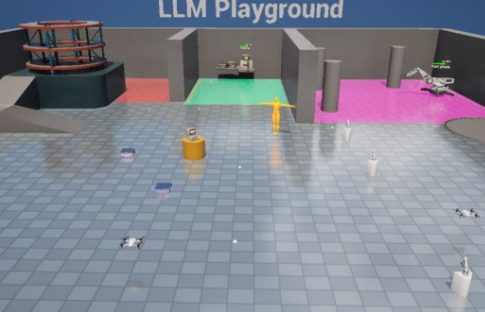
\includegraphics[width=0.5\textwidth]{figures/eval_env.png}
\caption{Simulation environment used for the evaluation process, showcasing color-coded rooms and functional areas.}
\label{simulation_environment}
\end{figure}
The evaluation process involved running the environment with 8 robots of different types, executing a comprehensive dataset of natural language commands ranging from simple to complex. Large Language Model (LLM) parameters, specifically temperature and top-p, were systematically varied at each iteration. At the conclusion of each episode, data was collected covering robot chat history, task results (success or failure), completion times, and additional relevant information. This data was then parsed and processed for further analysis, enabling assessment of robot cognitive performance under different environmental conditions and model parameters. Figure \ref{fig:evaluation_process} illustrates this evaluation workflow.
\begin{figure}[H]
\centering
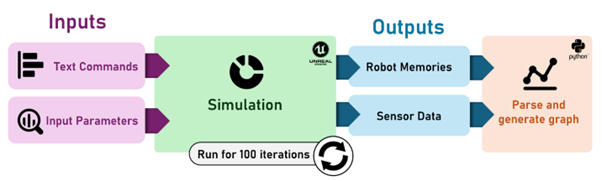
\includegraphics[width=0.8\textwidth]{figures/Picture4.png}
\caption{Diagram depicting the simulation evaluation process, from command input to data analysis.}
\label{fig:evaluation_process}
\end{figure}
To ensure a comprehensive evaluation, a varried collection of text commands was generated using techniques of synthetic data generation \cite{inproceedings}. These commands ranged from simple, structured sentences to more complex, context-dependent instructions, allowing for testing of the system's ability to handle varying levels of linguistic complexity.
The evaluation systematically explored different combinations of language model input parameters. To cover all possible combinations of temperature and top-p values (ranging from 0 to 1), the following equation was implemented:
\begin{equation}
(x, y) = \left(\left\lfloor\frac{i}{n}\right\rfloor \times 0.1, (i \bmod n) \times 0.1\right)
\end{equation}
where $x$ represents temperature, $y$ represents the Top-P value, and $n$ is the number of incremental steps for each parameter (set to 11, with increments of 0.1). This resulted in 121 distinct simulations, ensuring thorough exploration of the parameter space.
Following each simulation run, comprehensive data including chat histories, success rates, execution times, robot position data, and other relevant metrics were automatically saved in JSON format. A custom Python script was developed to parse and process these files from multiple simulation runs, facilitating automated evaluation of various key performance indicators.
This evaluation methodology aimed to strike a balance between operational efficiency and task success rates, assessing the effective integration of classical and modern techniques in enabling smooth human-robot collaboration on complex tasks.


\subsection{Task-Specific Performance}
Among the evaluated virtual robots (Table \ref{robot-performance}), the Explorer and Manipulator robots exhibited the highest success rates of 88.5\% and 82.3\% respectively, indicating strong performance in exploration and object interaction tasks. In contrast, the Communicator and Analyzer robots had lower success rates around 65\%, highlighting opportunities for improvement in complex communication and data analysis tasks.
Table 4.1: Robot performance values over all evaluation sessions.

\begin{table}[h]
\caption{Robot performance values over all evaluation sessions}\label{robot-performance}
\begin{tabular*}{\textwidth}{@{\extracolsep\fill}lcccl}
\toprule
Robot & Avg. Success Rate & Time (s) & Text Length (char.) & Most Used Ability \\
\midrule
Explorer & 88.5\% & 5.12 & 62 & Environmental Mapping \\
Manipulator & 82.3\% & 3.75 & 48 & Object Interaction \\
Communicator & 65.7\% & 4.21 & 89 & Robot Communication \\
Analyzer & 64.9\% & 3.98 & 71 & Data Analysis \\
Coordinator & 78.2\% & 0.00 & 156 & Task Assignment \\
\botrule
\end{tabular*}
\end{table}

When analyzing specific abilities, as shown in (Table \ref{ability-rating}), Object Manipulation emerged as the most successful with an 85.7\% success rate, demonstrating proficiency in physical interaction tasks. However, abilities like Complex Reasoning (62.1\%) and Multi-Agent Coordination (68.4\%) had comparatively lower success rates, indicating areas that require further enhancement.
Table 4.2: Average evaluation findings per ability.
\begin{table}[h]
\caption{Average evaluation findings per ability}\label{ability-rating}
\begin{tabular*}{\textwidth}{@{\extracolsep\fill}lccc}
\toprule
Ability & Success Rate & Average Time & Computational Resource Usage \\
\midrule
Environmental Mapping & 79.3\% & 4.86 & Medium \\
Object Interaction & 85.7\% & 3.52 & Low \\
Complex Reasoning & 62.1\% & 2.74 & High \\
Inter-Robot Communication & 71.5\% & 1.18 & Low \\
Multi-Agent Coordination & 68.4\% & 2.95 & Medium \\
Data Analysis & 73.2\% & 3.41 & Medium \\
\botrule
\end{tabular*}
\end{table}
\subsection{Parameter Optimization}
Success rates for robotic tasks were found to be significantly impacted by the top-p and temperature parameters used by the LLM (Figure \ref{heat-map}).
The analysis reveals optimal robotic planning performance occurs at intermediate levels of the top-p and temperature parameters, suggesting a balanced approach between exploitation and exploration is most effective. Notably, a temperature around 0.7 leads to high success rates, aligning with common LLM usage recommendations.
\begin{figure}[H]
\centering
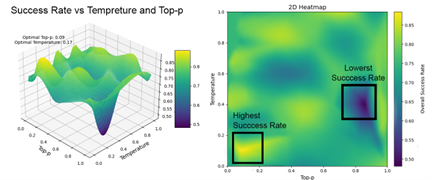
\includegraphics[width=0.9\textwidth]{figures/Picture1.png}
\caption{Success rate plotted against temperature and top-p sampling values.}\label{heat-map}
\end{figure}
The heatmap in (Figure \ref{spacial-map}) showcases the system's traversal and task allocation abilities across designated zones in the Unreal Engine environment.
The brightest trails indicate optimal routes for collaborative robot activities. Deviations suggest exploratory patterns for locating objects or obstacle avoidance behaviors.
\begin{figure}[H]
\centering
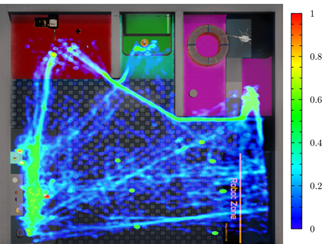
\includegraphics[width=0.5\textwidth]{figures/heatmap.png}
\caption{ Robot spatial Distribution and Activity Map}\label{spacial-map}
\end{figure}

\subsection{Running Cost and Scalability}
Figure \ref{running-cost} highlights the cost-effectiveness of the project's approach, proving very inexpensive for testing at a small scale while remaining manageable even as complexity increased. The cost trajectory highlights the methodology's affordable scalability, enabling comprehensive simulations and assessments without incurring prohibitive overheads.

\begin{figure}[H]
\centering
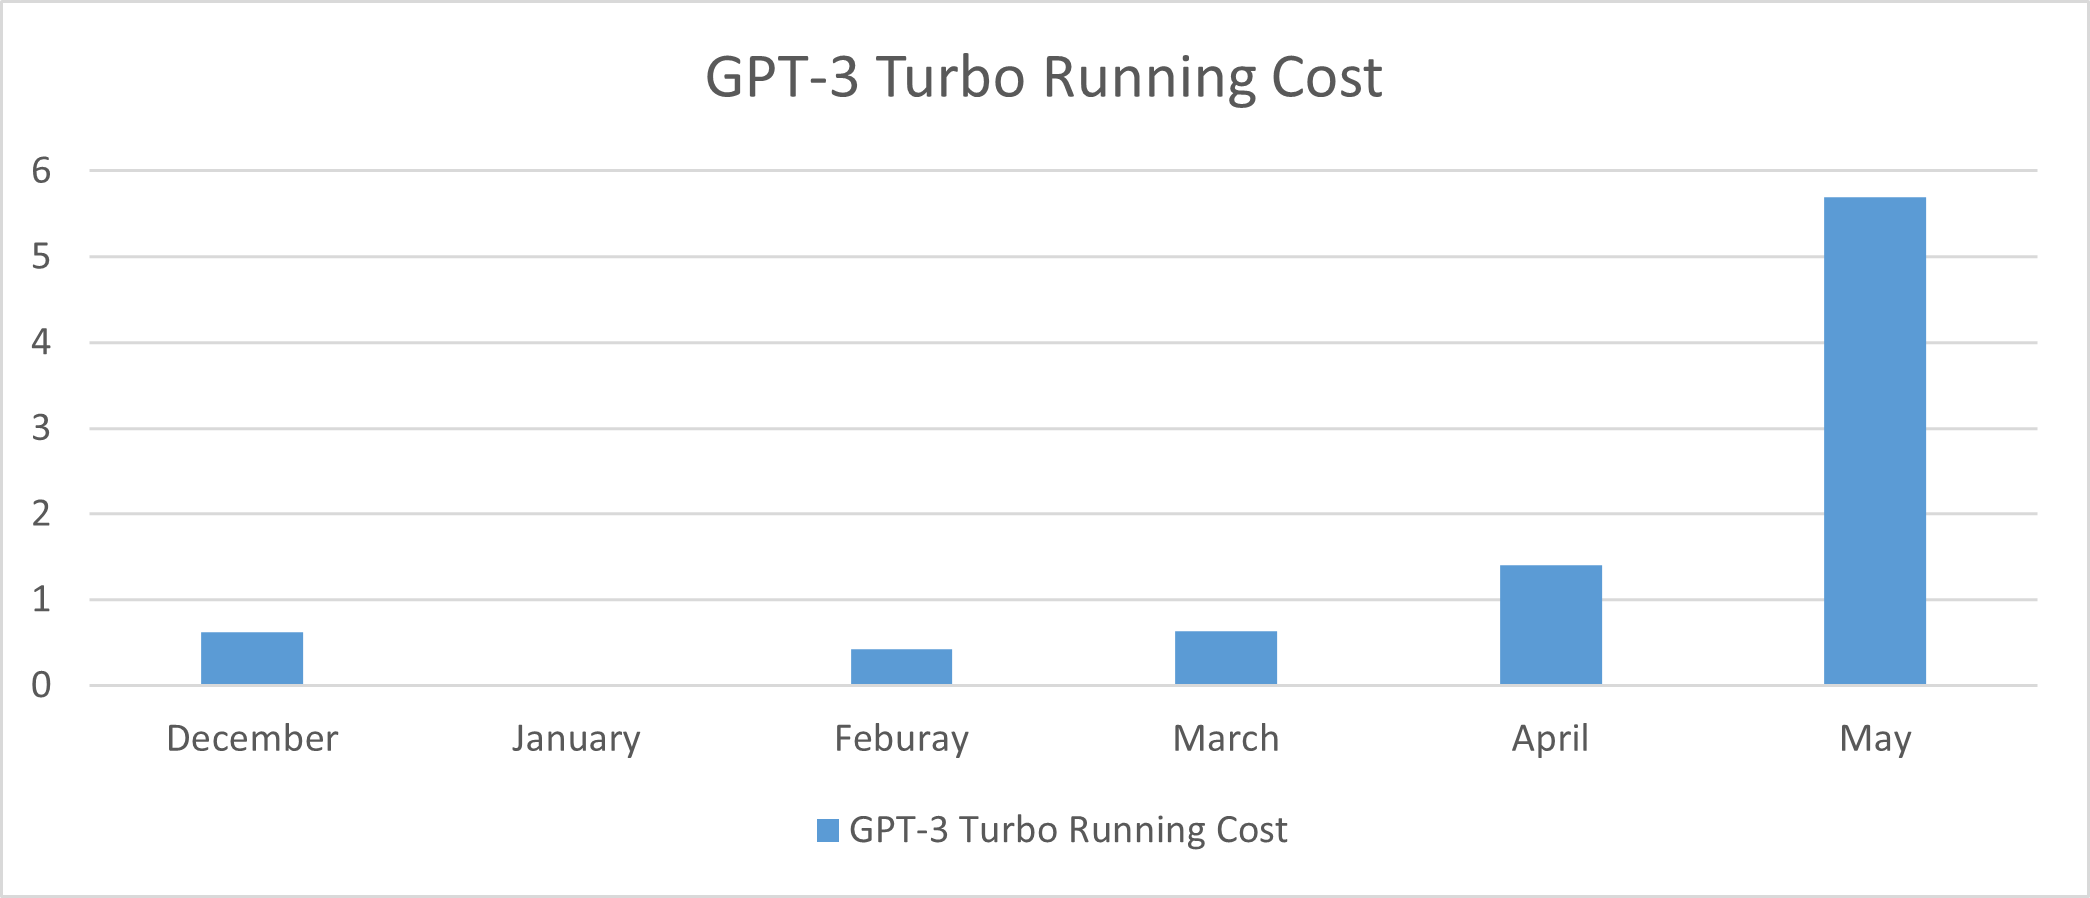
\includegraphics[width=0.8\textwidth]{figures/running_cost.png}
\caption{Language Model API Running Cost}\label{running-cost}
\end{figure}




\section{Conclusion and Future Work}


While LLMBot shows promise in bridging the gap between language understanding and robotic control, we acknowledge the challenges of balancing LLM capabilities with precise robotic control. Our modular architecture provides a flexible framework for future improvements, including integration with more advanced LLMs, sophisticated planning methods, and robust perception systems. \cite{brohan2023rt2}

As we look towards real-world applications, further research is needed to address the transition from simulated to physical environments. Despite these challenges, we are optimistic about the potential of LLMBot to pave the way for more intelligent, flexible, and reliable robotic systems across various domains.

\subsection{Limitations}
Language models can generate inaccurate or nonsensical outputs, known as hallucinations. These can lead to unintended behaviors, misinterpretations, false assumptions, and confabulation. Providing more context about the environment and grounding regarding the robot's abilities to the model can help mitigate hallucinations, but there is a trade-off between computational cost feeding the model more context and the risk of insufficient grounding.

\subsection{Future Work}
Key future enhancements include transitioning to the Robot Operating System (ROS) framework for real-world robotic hardware testing and deployment, integrating perception and navigation capabilities via real-life sensors, enabling system-generated general subroutines and action loops for task automation in factories and warehouses, and incorporating advanced planning methods other than behaviour trees like Hierarchical Task Networks (HTN) and GOAP (goal oriented action planning) for efficient execution of complex tasks. Future work should prioritize implementing these advanced planning techniques, ROS integration, and task queuing capabilities.


% \begin{figure}[H]
% \centering
% 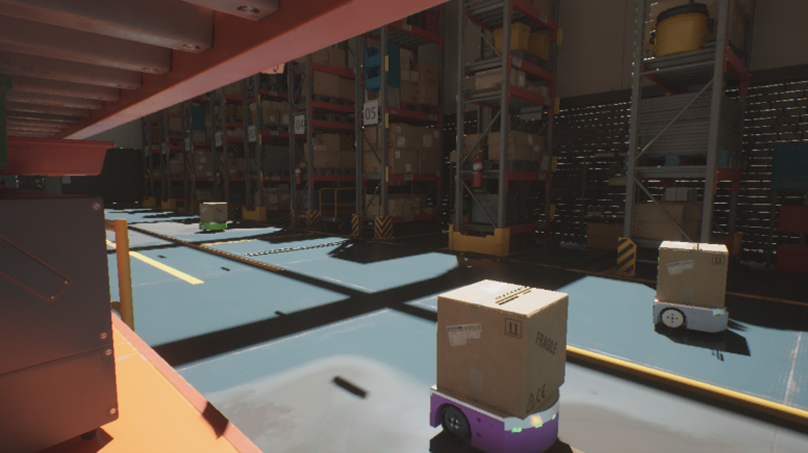
\includegraphics[width=0.6\textwidth]{figures/Picture10.png}
% \caption{Screenshot of the simulation. Intelligent robots managing inventory in a Warehouse.}\label{fig5}
% \end{figure}
% \begin{figure}[H]
% \centering
% 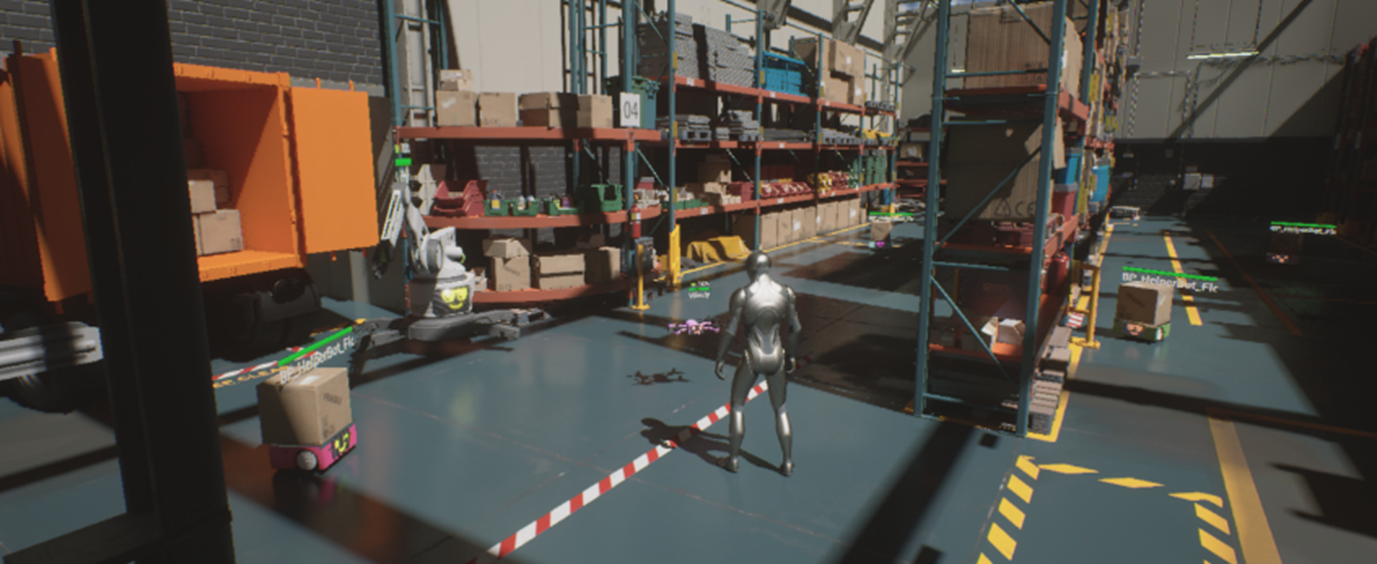
\includegraphics[width=0.6\textwidth]{figures/Picture14.png}
% \caption{Warehouse Simulation Environment in Unreal Engine 5.}\label{fig6}
% \end{figure}

\section*{Acknowledgments}
We would like to acknowledge the support of the University of Leeds for providing the resources and funding for this research project. We also express our gratitude to the staff of the School of Electrical and Electronics Engineering for their valuable contributions and insights throughout the project's development.




% \section*{Declarations}
% `Not applicable' 

% \begin{appendices}

% \section{Section title of first appendix}\label{secA1}

% An appendix contains supplementary information that is not an essential part of the text itself but which may be helpful in providing a more comprehensive understanding of the research problem or it is information that is too cumbersome to be included in the body of the paper. 

% \end{appendices}

\bibliography{sn-bibliography}



\end{document} 